One Sharp optical particulate sensor was tested against the EPA black carbon reference.  It was 1 month old at the time of installation, and ran for 59 days (from 4/15 - 6/13 2016) with two ~40 minute service interruptions.  This test gave 1,431 samples of hour resolution data.


\subsection{Pre-processing}

The Sharp sensor is a common choice for cheap air quality sensing projects, but is generally known as a simple device that can stuggle in outdoor conditions.  The signal from the sensor is a raw light magnitude, so to convert it to $\mu g/m^3$ requies an inversion and basic scaling.  After inversion, a LMSE optimization was applied against the reference sensor.  Instead of a straight LMSE algorithm, though, the cost function was modified to included only the values that were within 5\% of the reference signal.  This eliminates minimization errors due to regions where the sensors are mis-reading and mismatched.  This technique clearly out-performed the standard LMSE techniques tried (overall LMSE, LMSE without `outliers' more than one standard deviation away, etc).    This method worked well, and the sensor clearly followed the general trend of the EPA reference in many cases.  See Figure \ref{fig:sharpDust_lmse} for an example.

\begin{figure}[htb]
 	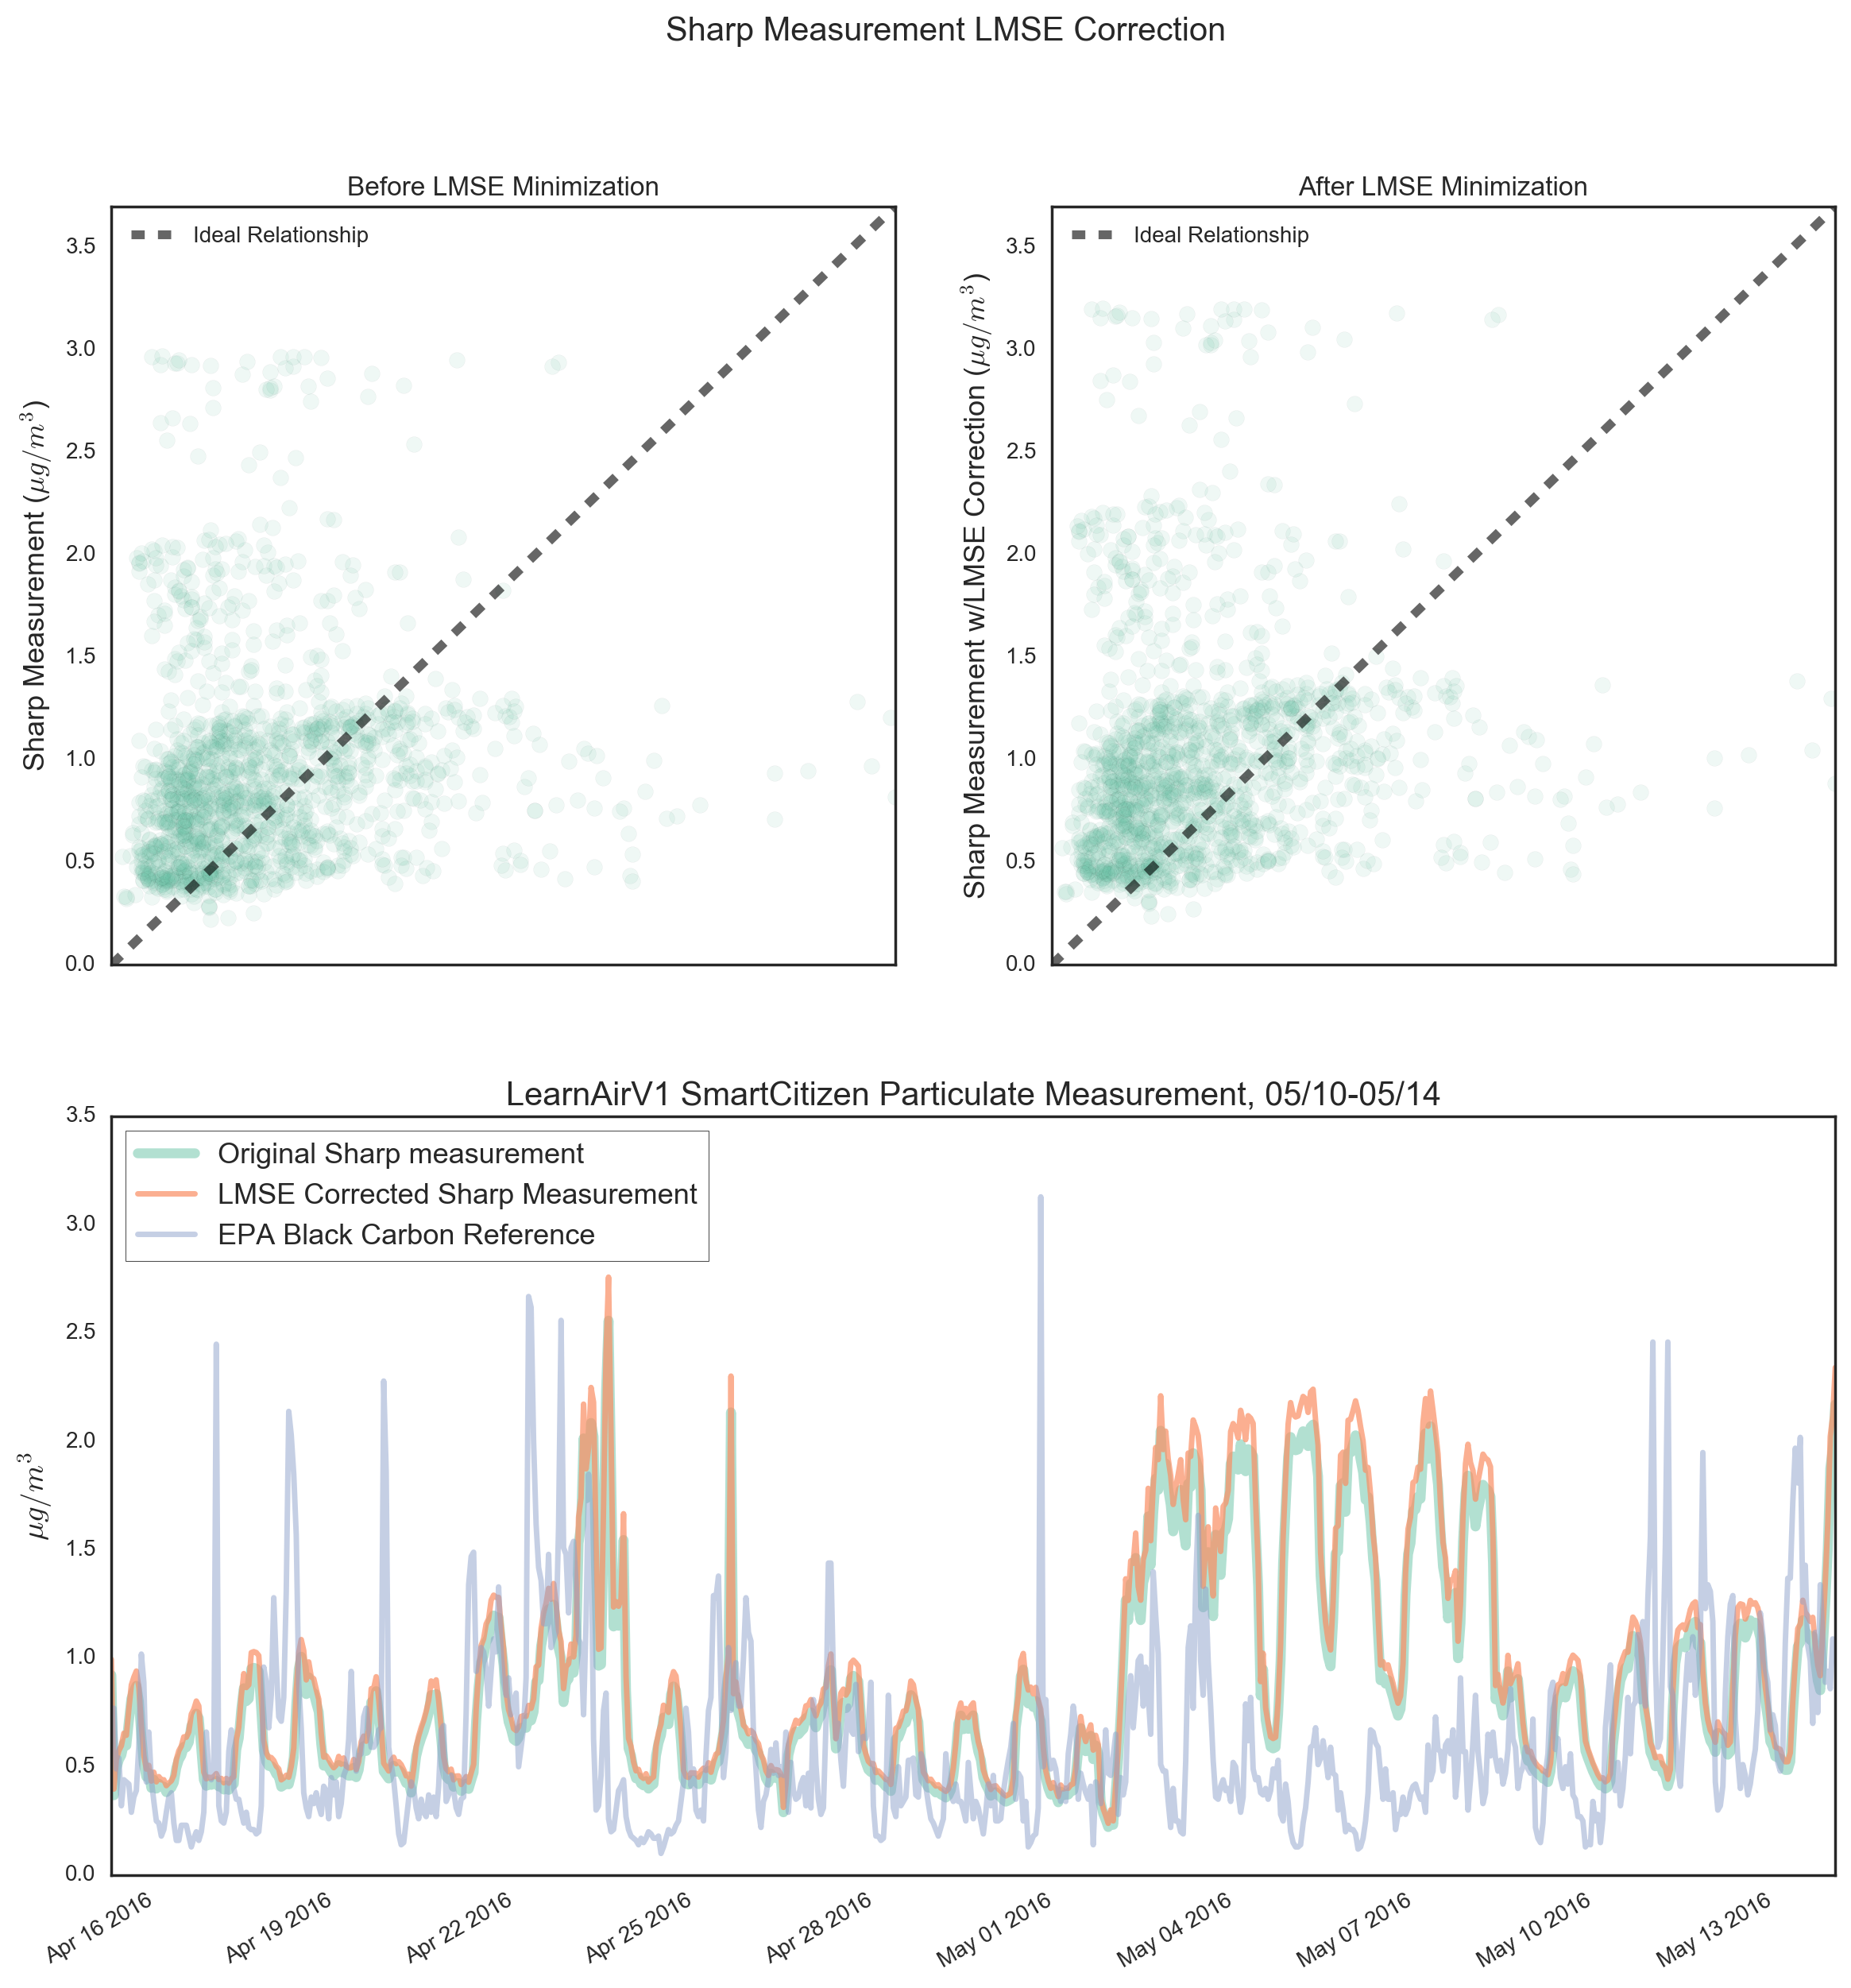
\includegraphics[width=\textwidth]{figs/sharpDust_lmse}               
 	 \caption{Sharp Particulate LMSE Calibration}
  	\label{fig:sharpDust_lmse}
\end{figure}

The reference sensor, for its part, labels readings in the following way: a `10am reading' of EPA sensor is recorded on filter paper from 10a-10:50a, then measured with an optical attenuation technique from 10:50-11a.  Thus, we averaged the 50 minute readings starting on the hour and threw away the last ten minutes.  After comparison, we added features with 6-, 12-, and 48- hour averaging.  The 48 hour measurement was also run through a LMSE process and used for machine learning (see Figure \ref{fig:sharpDust_avg_48_lmse}).

\begin{figure}[htb]
 	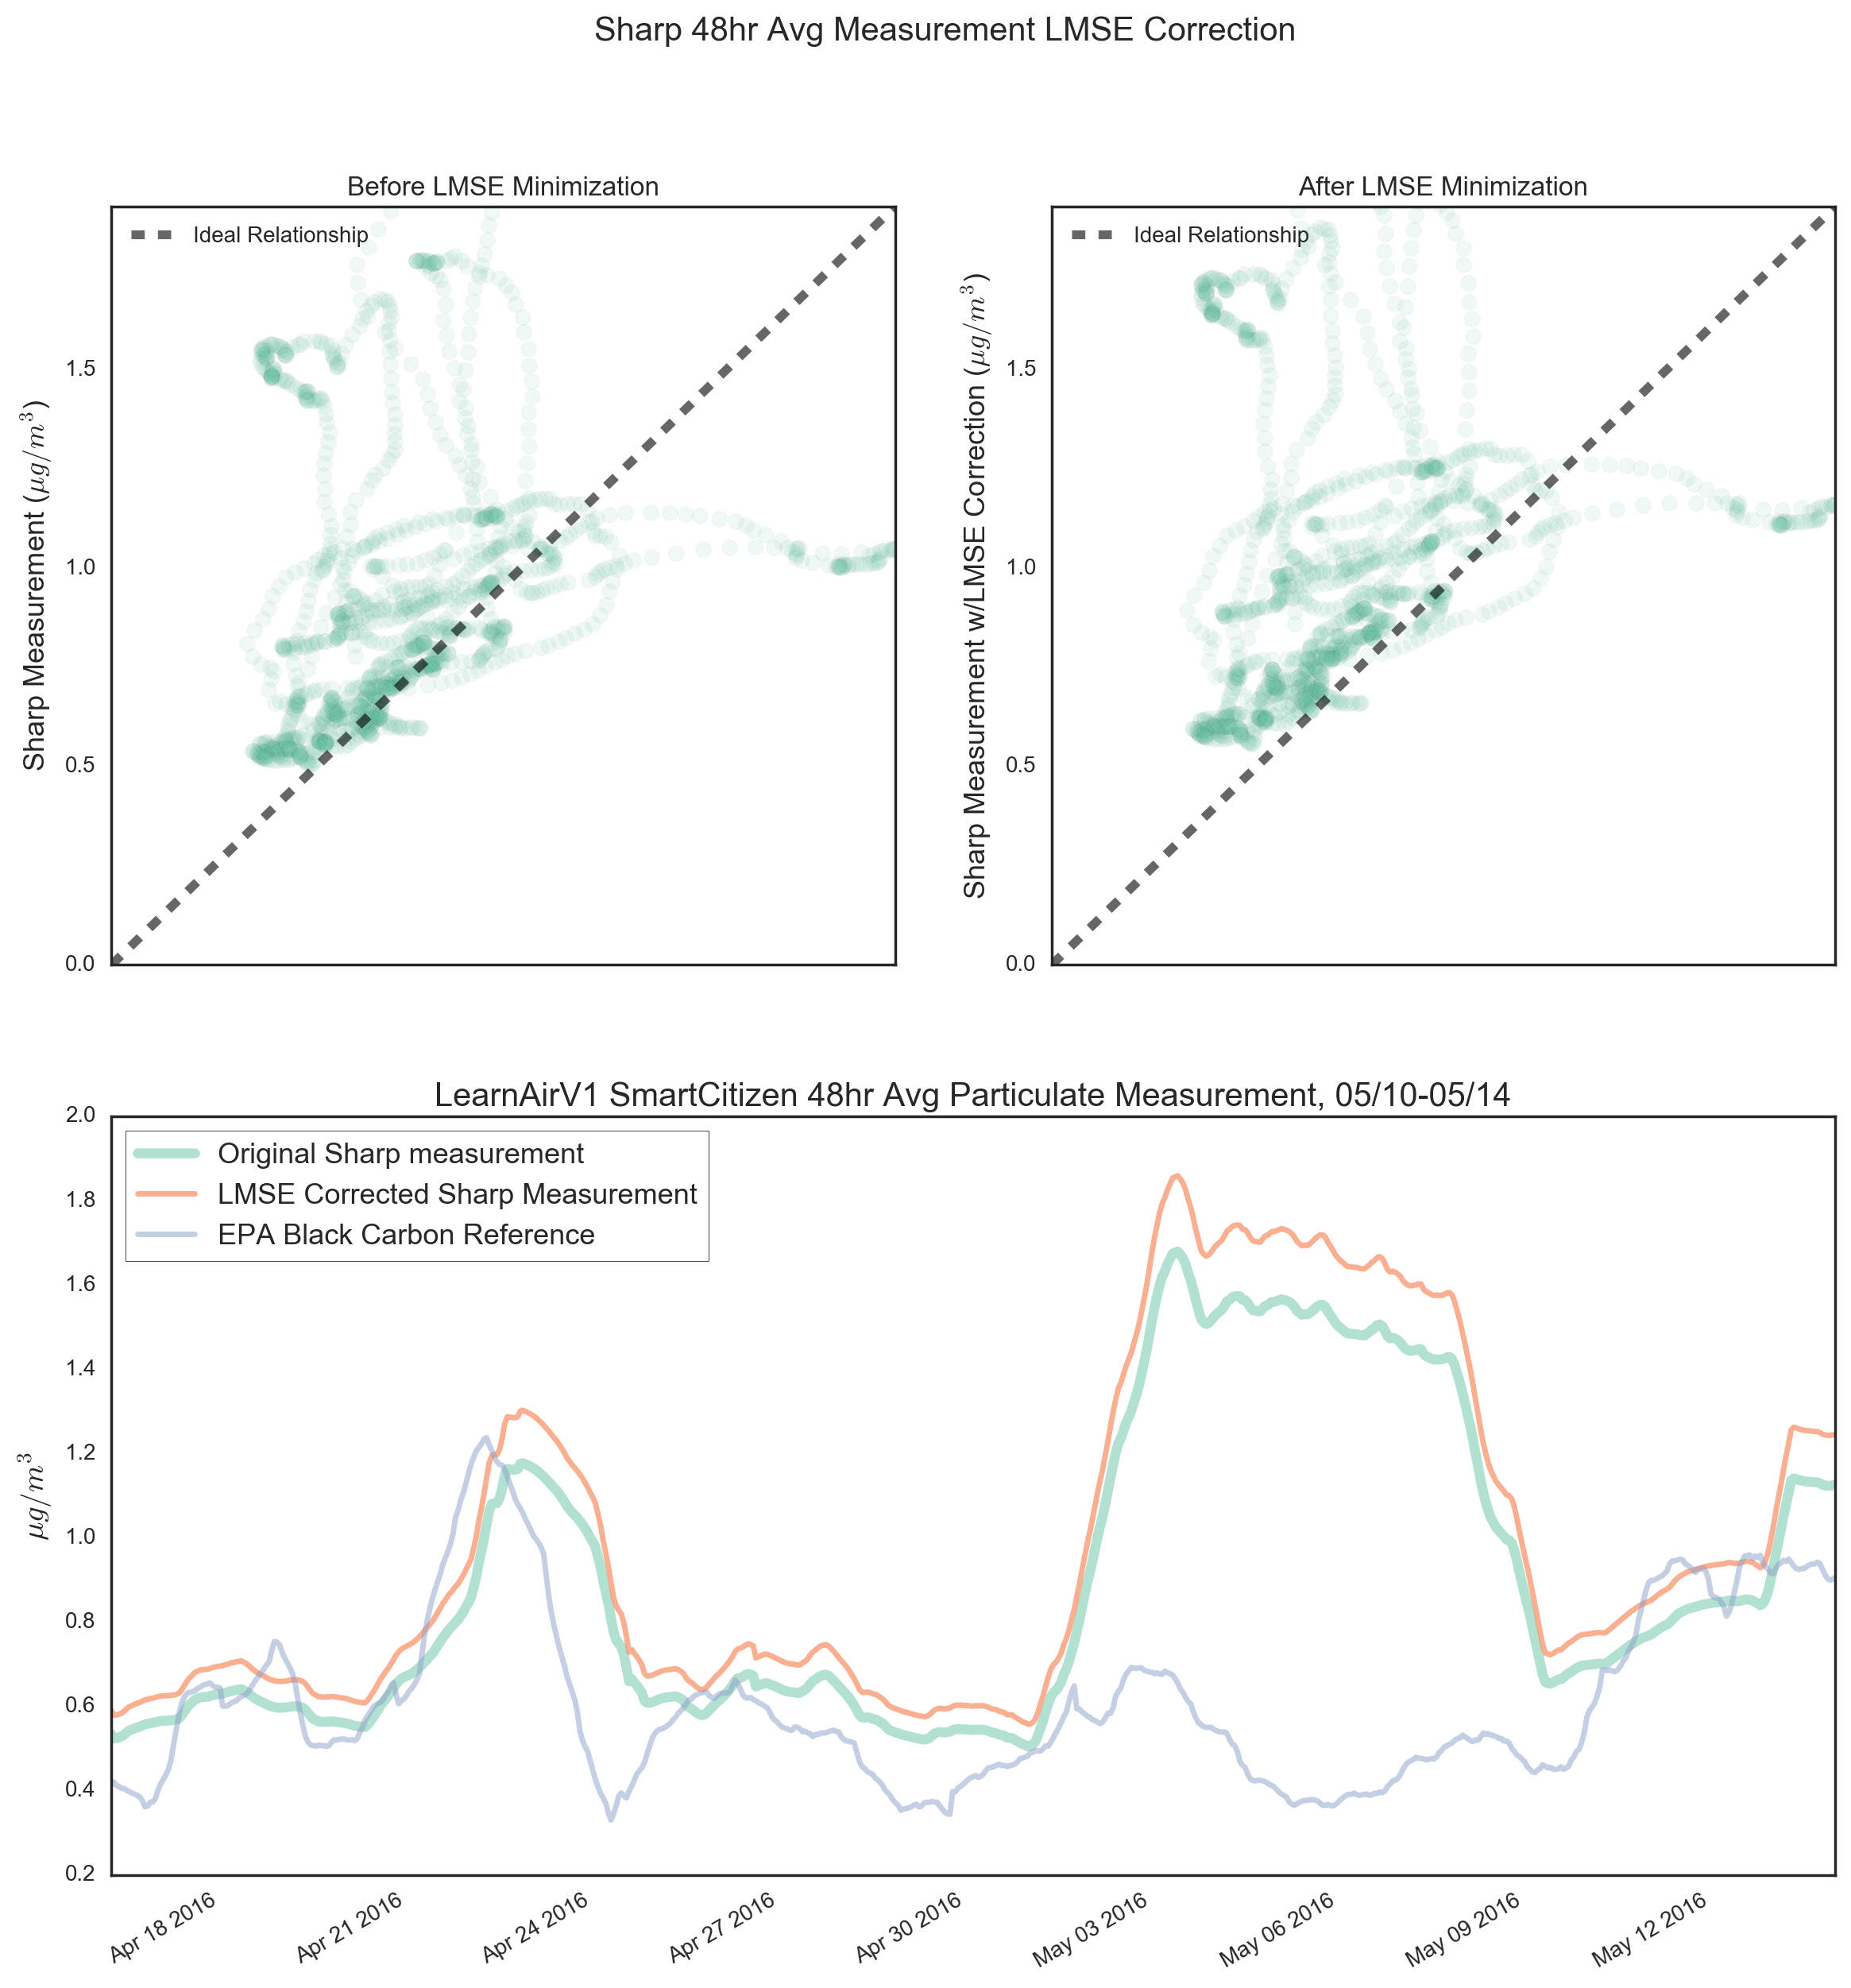
\includegraphics[width=\textwidth]{figs/sharpDust_avg_48_lmse}               
 	 \caption{2 day Average Sharp Particulate LMSE Calibration}
  	\label{fig:sharpDust_avg_48_lmse}
\end{figure}


\subsection{Machine Learning}

Machine learning on this data can provide us with useful insights about our ability to predict when the sensor works and when it does not.  The main test was run on errors using a 30\% tolerance-- 0.56 $\mu g/m^3$. Besides running our algorithm on the standard LMSE minimized signal, we also ran it using tried it using a 15\% tolerance (0.23$\mu g/m^3$), and 48-hr average with a 30\% tolerance based on its max value (0.29$\mu g/m^3$).  Figure \ref{fig:sharpDust_with_accuracy_zoomed} shows the main comparison with a 30\% accuracy overlay. 

Since this test uses hourly data, it is much faster to train and test a model.  It also means we have much less data to draw strong conclusions with.  In this case, we used a complete five fold validation to optimize our logistic regression parameter search of C = [0.001, 0.1, 10, 1000] and penalty-type=['L1', 'L2'].  We found the best parameters were C=1 with an L1 penalty.  For the tighter tolerance, an L2 penalty was more successful, and for the average values, C=10 worked best.

\begin{figure}[htb]
 	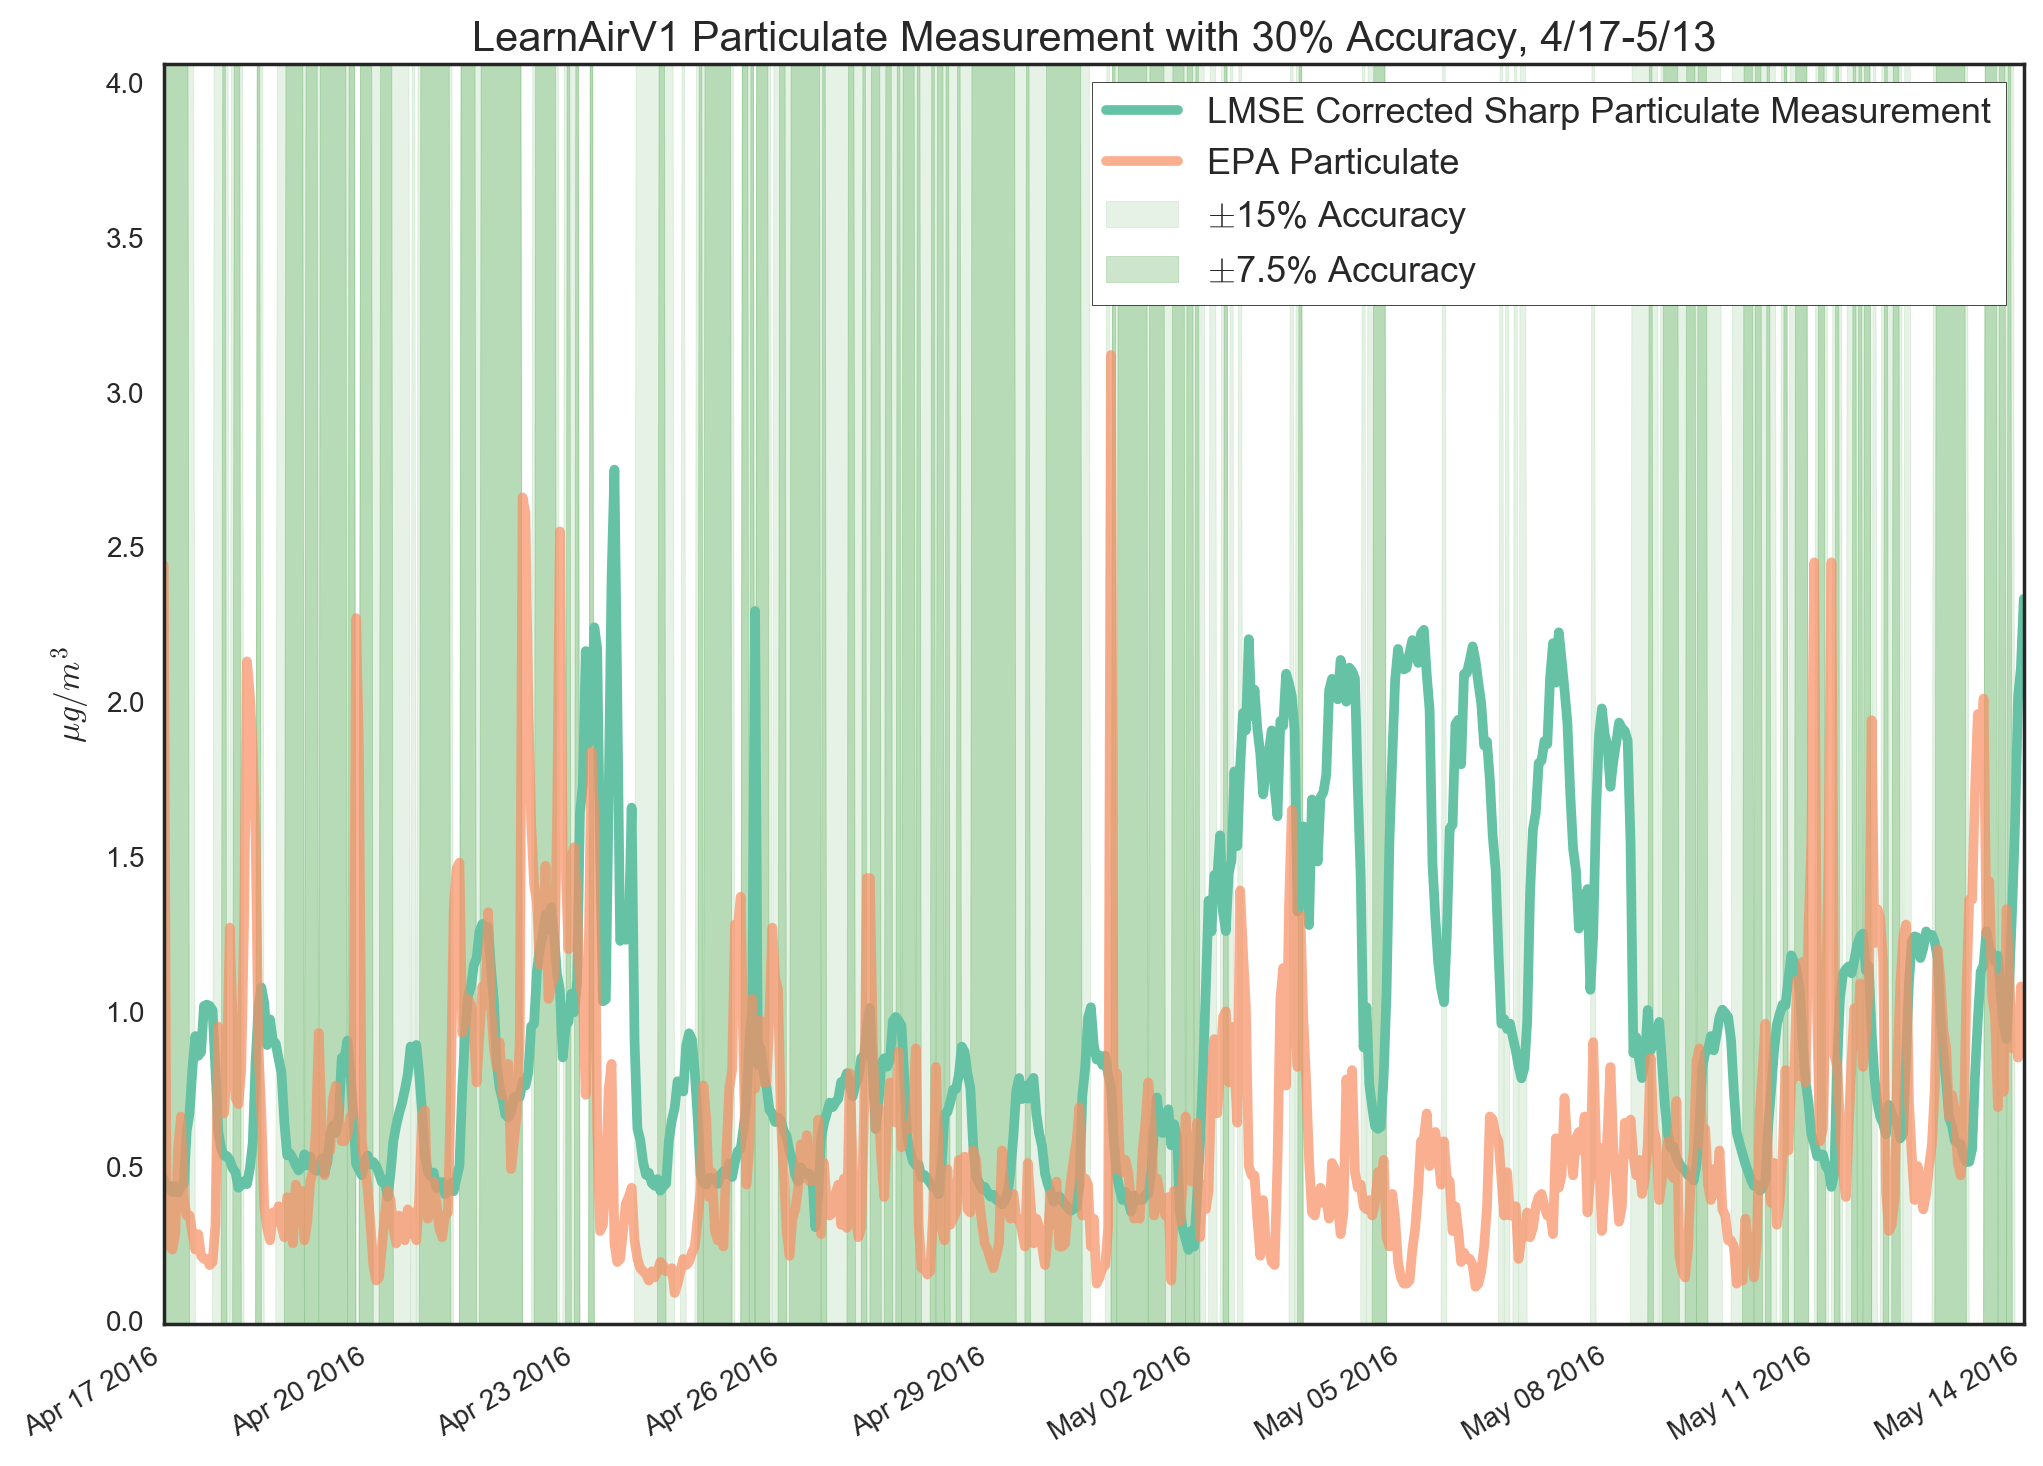
\includegraphics[width=\textwidth]{figs/sharpDust_with_accuracy_zoomed}               
 	 \caption{Sharp Particulate with 30\% Accuracy Threshold}
  	\label{fig:sharpDust_with_accuracy_zoomed}
\end{figure}

\begin{table}[]
\centering
\begin{tabular}{|c|c|c|c|c|}
\toprule
\multicolumn{5}{|c|}{Error Rates for CO Sensor #1 with Logistic Regression} \\
&\multicolumn{2}{|c|}{all features} & \multicolumn{2}{|c|}{top 15 features} \\
&shuffled & chunked & shuffled & chunked \\
avg & 0.17 & 0.22 & 0.22 & 0.25 \\
min & 0.14 & 0.18 & 0.20 & 0.14 \\
max & 0.20 & 0.29 & 0.24 & 0.36 \\
\bottomrule
\end{tabular}
\label{tab:sharp_error_rates}
\caption{Error Rates for Predicting Sharp Accuracy with Logistic Regression}
\end{table}

Error rates in Table \ref{tab:sharp_error_rates} show that we have a large difference between shuffled and chunked techniques, indicating we have no captured enough data to make fully seasonally robust predictions.  The error rates are also relatively high.

\begin{margintable}
\centering
\offinterlineskip
\hspace*{-5cm}\raisebox{-4cm}[0pt][0pt]{\rotatebox[origin=c]{90}{\parbox[c][0pt][c]{3cm}{\textbf{Actual Values}\\[20pt]}}}\par
\hspace{.3cm}\MyHBox[\marginparwidth]{Predicted Values}\par
\vspace{-.5cm}
\hspace*{1cm}\MyHBox{0}\MyHBox{1}\par
\MyTBox{0}{58.0}{35.2}
\vspace{-.35cm}\MyTBox{1}{14.0}{179.0}\raisebox{-1cm}
}
\label{tab:sharp_confusion}
\caption{Average Sharp Particulate Confusion Matrix w/Shuffled K-Fold}
\end{margintable}

Despite the high error rates, our AUC-ROC curve shows strong results (0.86 to 0.88 shuffled, 0.71 to 0.95 chunked)-- this suggests we're good at reporting the strength of our prediction (i.e., when we're wrong we reliably report the likelihood of a correct prediction close to 50\%, whereas when we're right we reliably report a likelihood closer to 100\%).  

\begin{marginfigure}
 	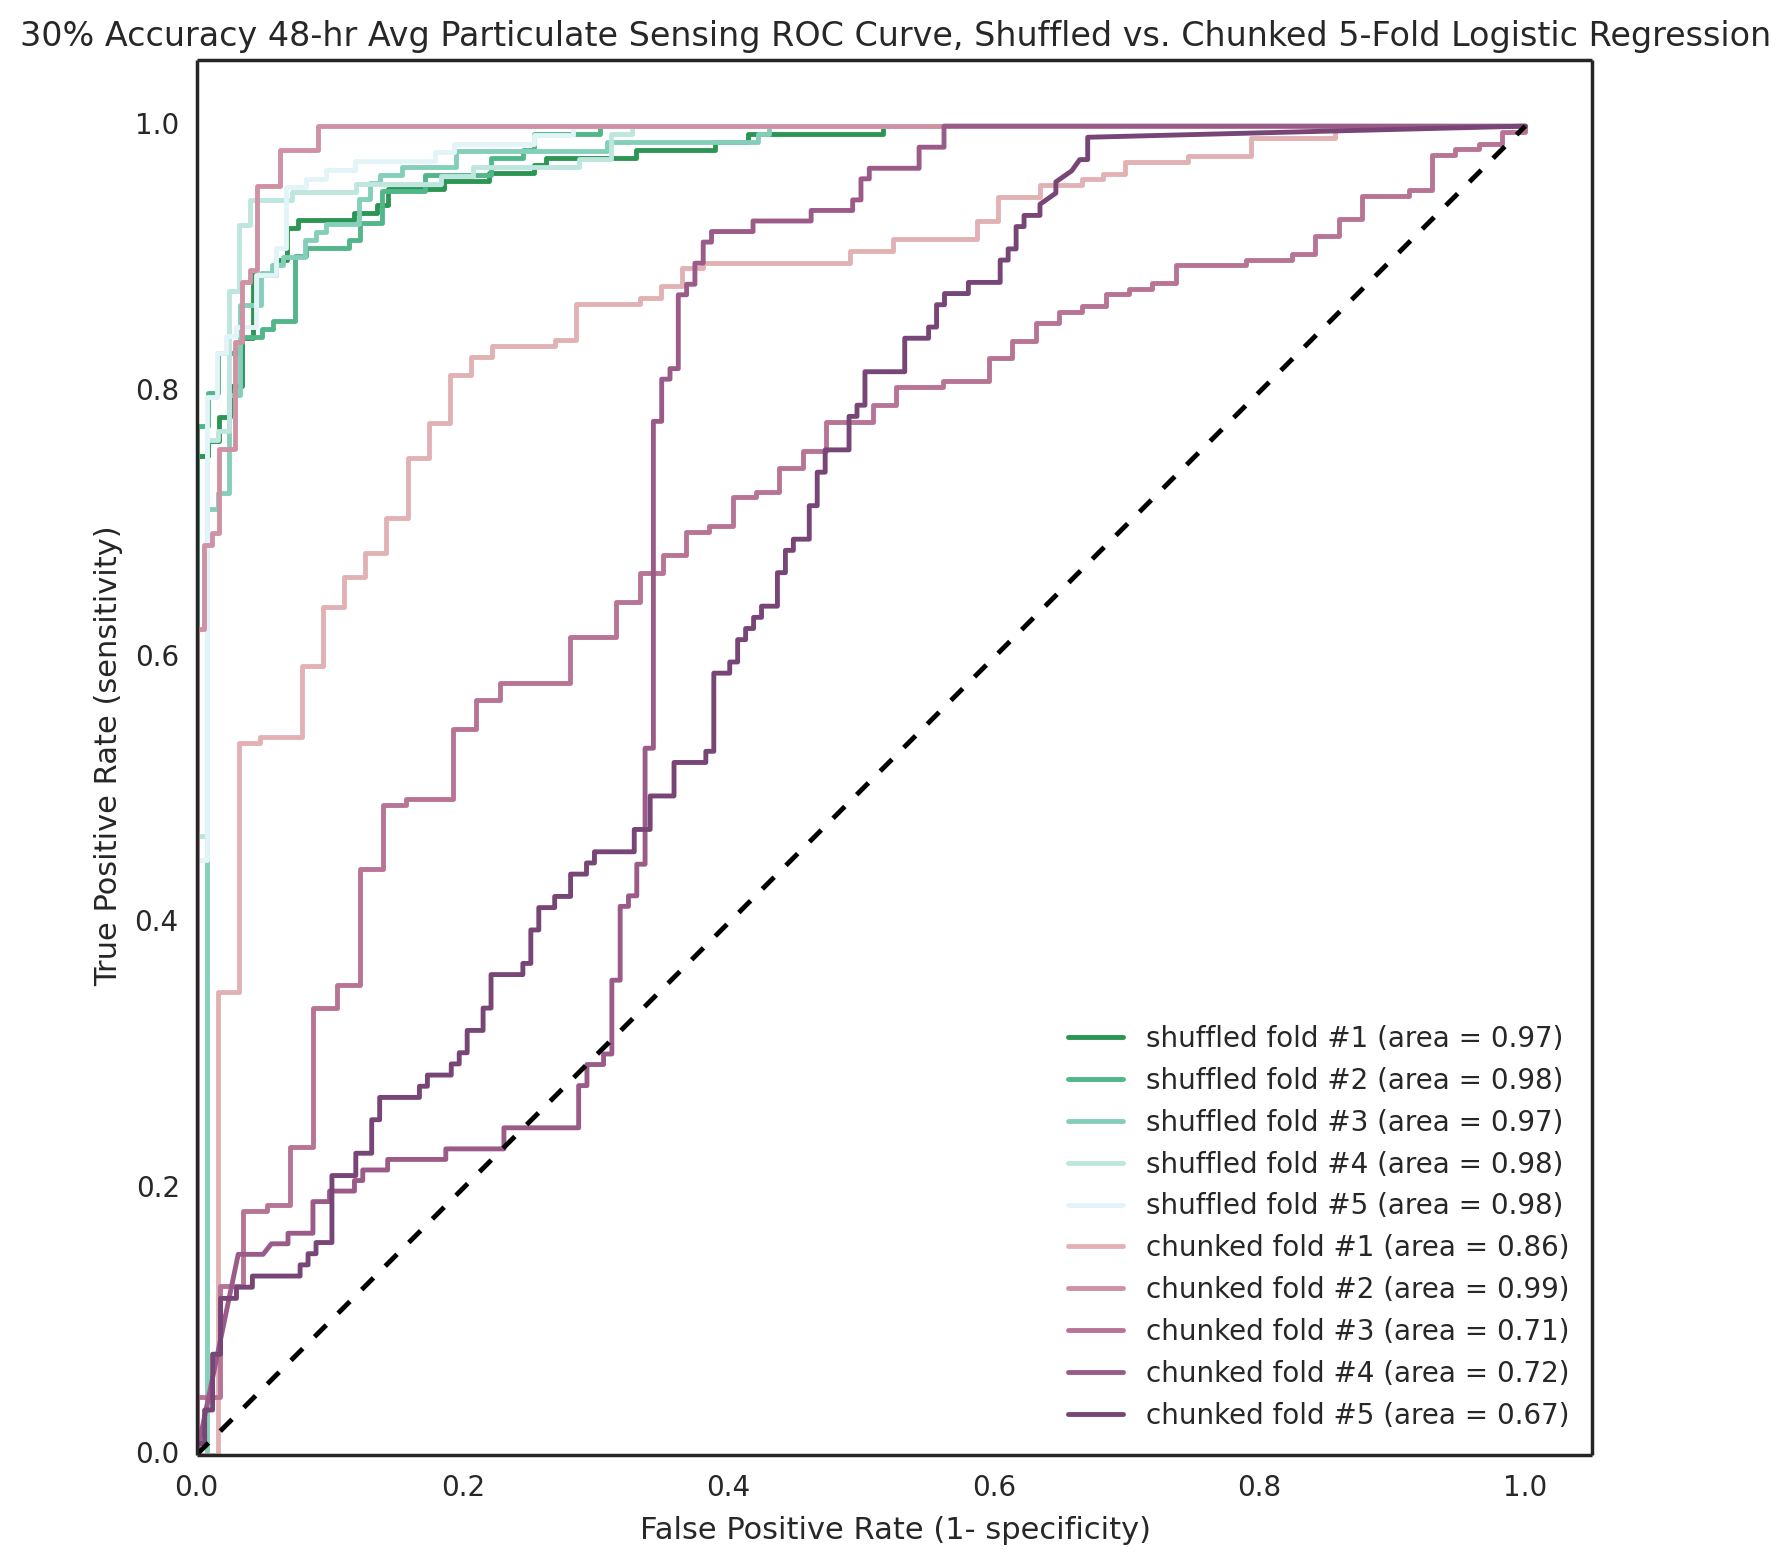
\includegraphics[width=\textwidth]{figs/sharp_48_avg_goals_30_roc}               
 	 \caption{48-hour Average Sharp Particulate ROC}
  	\label{fig:sharp_48_avg_goals_30_roc}
\end{marginfigure}

For 48-hour average data, we half the error rate in the shuffled case (down to 0.08), though the chunked case remains nearly the same.  (As a reminder, this is with a tighter absolute error tolerance as well, of $\pm$0.15 $\mu g/m^3$ instead of $\pm$0.28). We see dramatic results in the ROC curve for the shuffled case-- an average of 0.98 AUC-ROC.  These are very promising indicators that we can be extremely reliable in our prediction of certainty for each reading, especially with the averaged data.

\begin{figure}[htb]
 	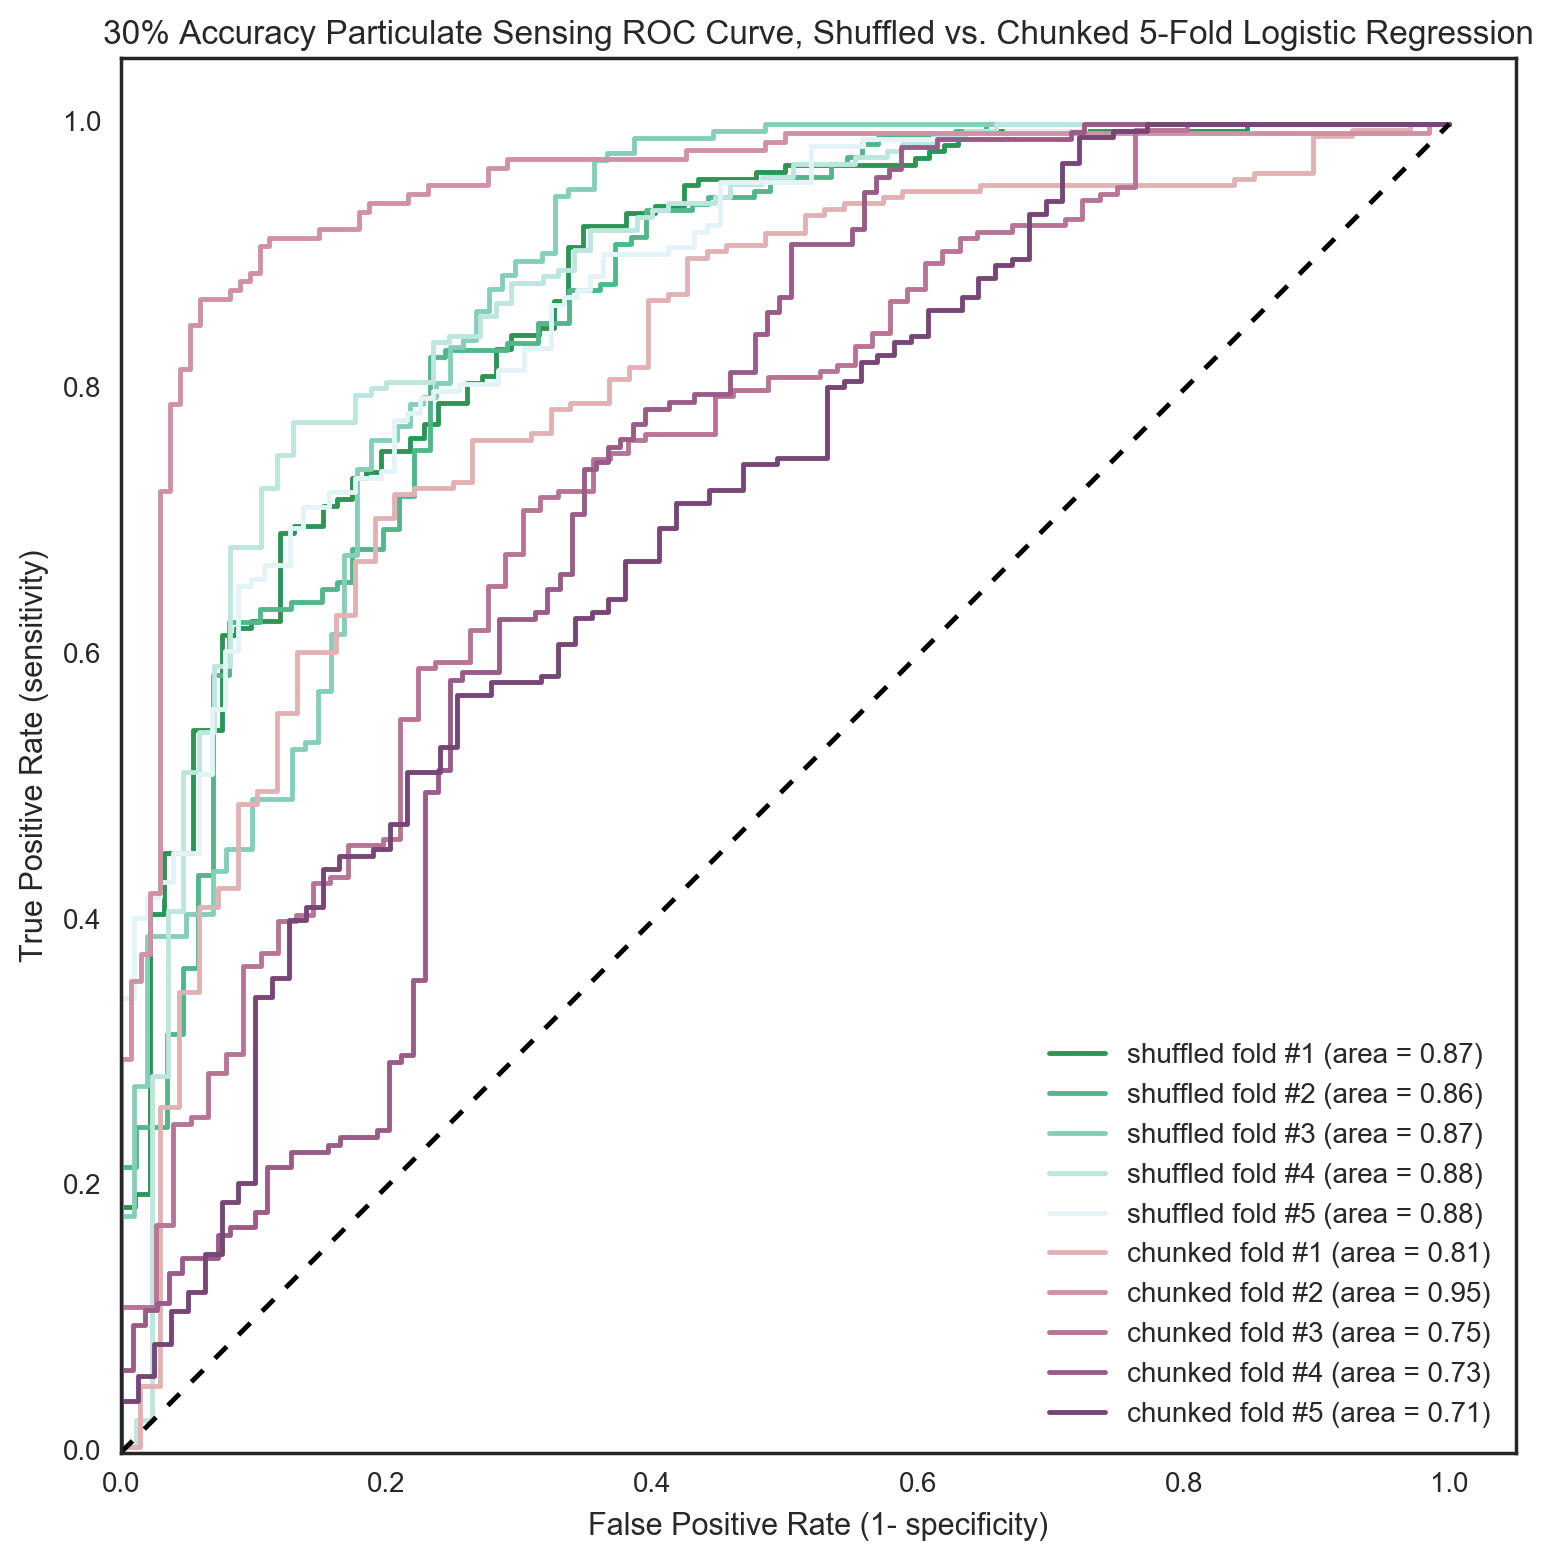
\includegraphics[width=\textwidth]{figs/sharp_goals_30_roc}               
 	 \caption{Sharp Particulate ROC Curve}
  	\label{fig:sharp_30_roc}
\end{figure}

It appears that our top 15 features do a relatively strong job on their own with these predictions, giving AUC-ROC values of 0.80-0.83 and 0.68-0.94 for the shuffled and chunked cases.  The top features for predicting particulate are derived from the Sharp sensor itself-- it appears that certain ranges of the sensor are more prone to error than others (high readings are less reliable).  The other top features (Table \ref{tab:sharp_top_features}) make sense given the physics of the device-- changes in NO2 seems to be a good indicator of sensor performance, as well as humidity level. (We would expect higher humidity to result in fog and condensation around particles that disperse light and increase reading error).  

These results are very promising.  They indicate extremely strong prediction performance, especially when comparing long-term averages.  They suggest we need to collect more data under more conditions before we are ready to predict across seasons.  There is one caveat, however.  In this test, the threshold for what is considered a `correct' measurement is quite high, at 30\% of the full range of observed values (0.6 $\mu g/m^3$ for the standard test).  This is a useful resolution, however it is a constrained choice.  When we cut this tolerance in half and retrain our models-- see Appendix D for more details-- the predictive quality starts to drop.  The effect of this threshold on predictive reliability of our model can provide an indication of sensor precision.  We can very accurately predict large errors with this sensor, but the inherent `noise floor' of the device limits that predictive strength as we tighten our tolerance.  
  

\begin{table}[]
\centering
\small
\begin{tabular}{lllllllll}
\\
\\
\toprule
     & Corr. & Lasso & Lin Reg & RF   & RFE  & Ridge & Stability & Mean \\
\midrule
sharpDust                                    & 1     & 0.65       & 0    & 1    & 0.81  & 0.03      & 1    & 0.64 \\
lmse\_scaled\_sharpDust                      & 1     & 0          & 0.03 & 0.65 & 0.83  & 0         & 0.98 & 0.5  \\
scaled\_sharpDust                            & 1     & 0          & 0.02 & 0.65 & 0.83  & 0         & 0.91 & 0.49 \\
avg\_12\_scaled\_sharpDust                   & 0.88  & 0          & 0    & 0.06 & 0.49  & 0.77      & 0.55 & 0.39 \\
derivative\_lmse\_avg\_15\_as\_no2           & 0     & 0          & 0.99 & 0    & 0.97  & 0.15      & 0.02 & 0.3  \\
derivative\_avg\_15\_lmse\_as\_no2           & 0     & 0          & 1    & 0    & 0.97  & 0.15      & 0.01 & 0.3  \\
derivative\_avg\_48\_scaled\_sharpDust       & 0.01  & 0          & 0.99 & 0.01 & 1     & 0.01      & 0    & 0.29 \\
derivative\_lmse\_avg\_48\_scaled\_sharpDust & 0.01  & 0          & 0.89 & 0.03 & 1     & 0.01      & 0    & 0.28 \\
temp\_as\_box\_differential                  & 0.01  & 1          & 0    & 0.22 & 0.47  & 0.13      & 0.05 & 0.27 \\
sck\_humidity\_saturated                     & 0.11  & 0          & 0    & 0    & 0.61  & 1         & 0.01 & 0.25 \\
Nitrogen Dioxide ( kOhm)                     & 0.18  & 0.06       & 0    & 0.02 & 0.72  & 0         & 0.67 & 0.24 \\
daily\_avg\_sck\_humidity                    & 0.24  & 0          & 0    & 0.05 & 0.6   & 0.69      & 0    & 0.23 \\
lmse\_sck\_no2                               & 0.18  & 0          & 0    & 0.02 & 0.72  & 0         & 0.67 & 0.23 \\
avg\_48\_scaled\_sharpDust                   & 0.45  & 0          & 0.02 & 0.01 & 0.88  & 0.18      & 0.07 & 0.23 \\
lmse\_avg\_48\_scaled\_sharpDust             & 0.45  & 0          & 0.02 & 0.01 & 0.87  & 0.2       & 0.06 & 0.23 \\
forecastio\_wind                             & 0     & 0          & 0    & 0    & 0.96  & 0.58      & 0    & 0.22 \\
derivative\_as\_no2                          & 0     & 0          & 0    & 0    & 0.99  & 0.57      & 0    & 0.22 \\
o3                                           & 0.1   & 0.25       & 0    & 0.06 & 0.14  & 0.01      & 0.85 & 0.2  \\
derivative\_Carbon Monxide ( kOhm)           & 0     & 0          & 0.36 & 0.03 & 0.99  & 0.01      & 0    & 0.2  \\
derivative\_lmse\_sck\_no2                   & 0     & 0          & 0.45 & 0.01 & 0.86  & 0         & 0    & 0.19 \\
derivative\_lmse\_sck\_co                    & 0     & 0          & 0.31 & 0.02 & 0.98  & 0.01      & 0    & 0.19 \\
daily\_avg\_forecastio\_humidity             & 0.29  & 0          & 0    & 0.02 & 0.46  & 0.41      & 0.05 & 0.18 \\
forecastio\_rain                             & 0.08  & 0          & 0    & 0    & 0.92  & 0.18      & 0    & 0.17 \\
alphaTemp                                    & 0     & 0          & 0    & 0.01 & 0.75  & 0.39      & 0    & 0.16 \\
\bottomrule
\end{tabular}
\label{tab:sharp_top_features}
\caption{Top Features for Predicting Sharp Particulate}
\end{table}


See Appendix D for more plots outlining the raw data, more information on the models with different accuracy thesholds and averaging, plots of the data with a correct/incorrect prediction overlay, and the Random Tree reduced-feature selection table and corresponding ROC curves. 
